\documentclass{article}
\usepackage{preamble}
\title{Constraint Solver Implementation}
\author{140011146}

\makeatletter
\let\thetitle\@title
\let\theauthor\@author
\let\thedate\@date
\makeatother

\begin{document}


\maketitlepage{CS4402 Constraint Programming}{Ian Miguel}




\section{Introduction}
In this practical, a forward checking constraint solver with 2-way branching is implemented. The implementation provides an interface to allow different heuristics for variable and value selection. To test the solver works as intended, problem instances of the N-queens, langfords and sudoku problems were generated and solutions created. Further, tests were written to ensure the right number of solutions were found for problem instances, for example exactly 724 solutions to the 10-queens problem. Finally, the performance of the solver and different heuristics are tested empirically using various metrics to explore and understand their differences. 

\section{Design and Implementation}
Many of the algorithms presented in this section were taken and adapted from the lecture slides to provide a complete method of what was done and any changes made during the implementation when compared to the original algorithm. 
\subsection{2 way forward checking}
The 2 way forward checking algorithm was implemented from the following algorithm:
\begin{algorithm}[H]
\begin{algorithmic}[1]
\Procedure{ForwardChecking}{\textit{varList}}
\If{completeAssignment()}
	\State addSolution()
\ElsIf{empty(\textit{varList})}
	\Return
\Else
	\State \textit{var} \gets selectVar(\textit{varList})
	\State \textit{val} \gets selectVal(domain(\textit{var}))
	\State branchFCLeft(\textit{varList}, \textit{var}, \textit{val})
	\State branchFCRight(\textit{varList}, \textit{var}, \textit{val})
\EndIf
\EndProcedure
\end{algorithmic}
\caption{2-way forward checking algorithm, adapted from lecture slides by Ian Miguel.}
\end{algorithm}
The small change made to the algorithm was to not exit when the first solution was found, but to add that solution to a list and continue to find more solutions. This was done to allow all solutions to be found as a means of testing the solver is working properly.
% A boolean variable was also added to stop the solver on the first solution found if needed. This was important to be able to experiment on the differences between finding one solution and finding all solutions, especially for larger constraint problems. 
To check for \texttt{completeAssignment()}, all variables in the problem instance contained a boolean to indicate that they have been assigned. \texttt{completeAssignment()} is true if all the variables are assigned. The variables can further be unassigned later by changing the assignment boolean in the corresponding variable.  
\n
The two methods \texttt{selectVar()} and \texttt{selectVal()} are implemented using heuristics which are explained below in section \ref{sec:heuristics}. Each heuristic implements its own variable and value selection functions which the solver uses, allowing the solver to be generic and extensible over any heuristic. Further, this means the heuristics do not have to worry about any other part of the solver, as the list of variables and domain of values are updated and kept track of in the solver to be passed to the heuristics. 
\n
Next, we look into detail on the algorithms for left and right branching.
\begin{algorithm}[H]
\begin{algorithmic}[1]
\Procedure{branchFCLeft}{\textit{varList}, \textit{var}, \textit{val}}
\State assign(\textit{var}, \textit{val})
\If{reviseFutureArcs(\textit{varList}, \textit{var})}
	\State ForwardChecking(\textit{varList} - \textit{var})
\EndIf
\State undoPruning()
\State unassign(\textit{var}, \textit{val})
\EndProcedure
\end{algorithmic}
\caption{Branching left during forward checking.}
\end{algorithm}
When we branch left, the selected value is assigned to the selected variable and future arcs revised. The idea is to ensure that for any particular value assignment, the arcs are revised to ensure local arc consistency. If the arc is still consistent, then we explore further down the tree by recursively forward checking with the reduced list of variables.
\n
When the functions eventually return or if the arc is inconsistent, the current value assignment does not lead to a solution, so any pruning done during arc revision must be undone for backtracking as the value assignment has not worked out. This is done with the \texttt{UndoTracker} class which keeps a map of each variable and the list of pruned values that need to be undone. Next, the solver contains a map of each variable to an \texttt{UndoTracker}. Whenever arcs are revised, the tracker for the variable chosen for revision is updated with the list of other future variables and their pruned values. This works to prune only values from each step of the recursion, because every time the algorithm goes down the left branch, a new variable is selected to be assigned and its arc revised. So when coming back up the tree, each depth corresponds directly to the selected variable, which acts as the key to an \texttt{UndoTracker}. 

\begin{algorithm}[H]
\begin{algorithmic}[1]
\Procedure{branchFCRight}{\textit{varList}, \textit{var}, \textit{val}}
\State deleteVal(\textit{var}, \textit{val})
\If{\neg\ empty(domain(\textit{var}))}
	\If{reviseFutureArcs(\textit{varList}, \textit{var})}
		\State ForwardChecking(\textit{varList})
	\EndIf
	\State undoPruning()
\EndIf
\State restoreVal(\textit{var}, \textit{val})
\EndProcedure
\end{algorithmic}
\caption{Branching right during forward checking.}
\end{algorithm}
As this is a 2-way branching scheme, the right branch is the branch where the given value assigned on the left branch is now removed. This removed value in \texttt{deleteVal()} does not have to be stored or kept track of as the same value is passed to the \texttt{restoreVal()} method later in the same function scope. Future arcs are revised again before any further forward checking and of course the pruning is undone afterwards as well.
\n
Finally are the algorithms for revising arcs. The algorithm for \texttt{reviseFutureArcs()} is not shown, as it remains unchanged. For all variables passed into it, the arc between the currently assigned variable and the list of future variables is revised and if the local arc consistency is broken at any stage, the function returns false. The method for which each arc is revised is detailed as follows:

\begin{algorithm}[H]
\begin{algorithmic}[1]
\Procedure{Revise}{\textit{Arc($var_1$, $var_2$)}}
\State \textit{val} \gets $var_1$.assignedValue()
\State \textit{constraints} \gets getArcConstraints(Arc($var_1$, $var_2$))
\If{empty(\textit{constraints})}
	\Return False
\Else
	\For{each constraint \textit{c} in \textit{constraints}}
		\For{each value \textit{v} in domain($var_2$)}
			\If{$\neg$\ constraintHolds(\textit{c}, \textit{v})}
				dropVal($var_2$, \textit{v})
			\EndIf
		\EndFor
	\EndFor
\EndIf
\EndProcedure
\end{algorithmic}
\caption{Algorithm for revising an arc.}
\end{algorithm}
There were a few difficulties encountered during the implementation of the revision step. First, because of the way the assigned values are implemented in any given variable, if a variable has been assigned, \texttt{revise()} only uses the assigned value to revise the arcs to all other variables. This means to deal with revision during right branching, the revision function has to be altered to revise for each value in the variable's domain. A more streamlined way to handle this would have been to represent assigning a value by only leaving the assigned value in the domain of the chosen variable. That way the same code can be reused for both left and right branching, as both options loop through all values in the variable's domain. The second issue was an issue with the way the \texttt{.csp} constraint problems were written and parsed. In the \texttt{.csp} format, an arc is specified both ways under one \texttt{BinaryConstraint} which contains both variables. 
\begin{lstlisting}[caption={Example of how constraints are specified in \texttt{.csp}}]
c(0, 1)
1, 3
2, 4
3, 5
4, 6
\end{lstlisting}
In the above listing, the tuples in constraint \texttt{c(0, 1)} applies both ways and have to be matched accordingly, rather than simply being the arc in the direction arc($v_0$, $v_1$). For example if the selected variable was $v_1$, the second value of the tuples have to be used rather than the first. The change needed to implement this was to keep a copy of the tuples reversed so that when matching to the constraint, the reversed tuples can be returned if that order is needed (i.e, checking the arc($v_1$, $v_0$) rather than the arc ($v_0$, $v_1$). 
\n
Furthermore, there is a distinction between no arc existing between two variables and no constraints in an arc between two variables. An example of the first case is common in Sudoku problems, where two cells that don't share the same row, column or grid do not have an arc between them as they do not affect each other. An example of the latter case is in the 2-queens problem, where there are no constraints specified between the first and second row, because there are no valid values for either. This was a case that had to be handled carefully, as the arcs are still consistent if no arc exists between two variables, but the arc not consistent if there are no valid values for the arc, as in the 2-queens problem. 

\subsection{Heuristics}\label{sec:heuristics}
The heuristics used for the solver are implemented as an abstract class to allow any additional heuristic to be easily implemented. The class exposes three functions for any subclass implementations:
\begin{itemize}
\item \texttt{getNextVariable(\textit{varList})}
\item \texttt{getNextValue(\textit{varDomain})}
\item \texttt{toString()}
\end{itemize}
The first two allow any implementation of a heuristic to choose the next variable and value that should be returned from the list of variables and domain of values. The \texttt{Heursitic} abstract superclass implements a default behaviour which returns the first element from the list of variables and domain values. This further allows a heuristic implementation to choose to only implement the choice of variables, value or both and default to choosing the first element otherwise. For example, the heuristic \texttt{RandomValueHeuristic} chooses the next value randomly from the domain, but uses the default behaviour of the superclass to choose variables. 
\n
The \texttt{toString()} method simply gives a name for the heuristics to easily identify them for data gathering reasons. 

\subsubsection{Static variable heuristics}
A few simple static variable ordering heuristics were used:
\begin{itemize}
\item \textbf{Ascending order} - The static ascending order heuristic is the default heuristic which always chooses the first element in the list of variables. 
\item \textbf{Descending order} - Order of the variables are chosen in descending order. For example if there were 3 variables $v_{1}, v_{2}, v_{3}$ the order for choosing variables becomes $v_{3}, v_{2}, v_{1}$. 
\item \textbf{Odd/even order} - All odd numbered variables are chosen first, then even numbered variables. The variables are further chosen in ascending order. For example, given 5 variables $v_{1}, v_2, v_3, v_4, v_5$, the chosen order becomes $v_1, v_3, v_5, v_2, v_4$. 
\item \textbf{Maximum degree} - Choose variables which are the most constrained first, as they are likely to be the hardest choices. This was done by calculating the total number of possible value combinations between each pair of variables minus the number of tuples between the pair from the CSP description. This gives the total number of constraints for one variable to all other variables. The variables are sorted and chosen by highest number of constraints first. 
\item \textbf{Minimum degree} - Simply the opposite of maximum degree, where the variables with the \textit{least} number of edges in the primal graph are chosen first. This heuristic was implemented to show that the opposite behaviour of maximum degree performs more poorly.
\end{itemize}
For all these variable heuristics, the values from the domains are chosen in ascending order as the domain is stored as a sorted set, so the first value chosen is the lowest one. 

\subsubsection{Dynamic heuristics}
The only dynamic heuristics implemented was smallest domain first and its inverse (largest domain first). These were done by checking the domain of each variable in the list of variables and choosing the one with the smallest or largest number of domain values. 

\subsubsection{Random heuristics}
Random heuristics were implemented for empirical testing to see how they would perform if a random variable or value assignment was chosen on every step. The three different random heuristics (\texttt{Random}, \texttt{RandomVariable} and \texttt{RandomValue}) also allow us to see the difference between variable and value heuristics. \texttt{Random} randomly chooses both variable and value, while \texttt{RandomVariable} and \texttt{RandomValue} only choose the variable and value respectively as their name implies. The random nature of these heuristics combined with many iterations should be able to show any differences between choosing the variable and value, showing if one may impact performance more than another. There is also a fourth \texttt{RandomStatic} heuristic, which statically chooses the random order at the beginning rather than choosing randomly every step. This is subtly different from a dynamic random order because each left subtree that is explored will stay in the same random order, whereas choosing randomly dynamically will change every subtree to be different and random. 

\section{Experimental methodology}

\subsection{Testing}
To make sure that the constraint solver worked as intended, JUnit tests were written. Because the constraints problems and solutions can be very large, it was not feasible to write tests that checked the correctness of all solutions. However, smaller problems such as the 4Queens problem could be tested. Furthermore, the solver can be specified to output all solutions in which case the number of solutions (including all symmetrical solutions) can be tested to ensure the correct number of solutions were found. 
\n
Further, tests were written for each heuristic to make sure each heuristic was not doing anything wrong that changed how the solver worked. 

\subsection{Metrics used}

Multiple metrics were used to empirically measure the performance of different heuristics. Time, number of solver nodes and number of arc revisions were all used as metrics. The number of solver nodes was calculated as the number of times \texttt{forwardChecking()} was called and did not return immediately as it represents a step down into the recursion and search tree. The number of arc revisions was calculated each time a constraint between two variables was revised. For example, if there are two variables and two and three values in their domains respectively, the number of arc revisions between one variable to another is 6. Finally the time taken only takes into account the time the solver took to solve the problem and find all solutions rather than the total time of the whole process. 
\n
The three metrics were all chosen for various reasons:
\begin{itemize}
\item \textbf{Solver nodes} - The number of solver nodes tells us how large of a search tree had to be explored in order to find the solutions. If different heuristics give different numbers of search nodes, it tells us that the heuristic had to do more or less searching by giving the size of the search tree. Because all solutions are found in our experiments, the search does have to be exhaustive. However, a more effective heuristic would prune more domain values earlier in forward checking and therefore have a smaller search tree with less nodes. 
\item \textbf{Arc revisions} - The reason the number of arc revisions was measured is similar to why solver nodes is  measured. The number of arc revisions give an even more detailed look at how much work is being done at each node of the search tree. Had an algorithm like AC3 been implemented, the number of arc revisions would also help in differentiating the different between forward checking and maintaining arc consistency, as it would cost more revisions to maintain arc consistency, but search less nodes. 
\item \textbf{Time taken} - The time taken was chosen because ultimately an important aspect of solvers is how long it takes. A complicated algorithm could solver constraint satisfaction problems in fewer revisions and search nodes, but take a lot of time, so it is still valuable to measure the time needed. 
\end{itemize}

\subsection{Experiments}
Multiple runs of the experiments were done to ensure reliable results for using the random heuristics. The number of search nodes and revisions do not normally require multiple iterations because they are deterministic, so every run would lead to the same resulting number of arc revisions and solver nodes. However a random heuristic that randomly chooses the next variable to assign would require the extra runs to determine an average number of nodes and arc revisions. Furthermore, because the time taken was also measured, the additional runs were needed to find an average time. Because of time benchmarking issues in Java due to the JVM \cite{jvm-benchmark}, the time taken is not unreliable without a robust benchmarking framework. 
\n
To run the experiments, an \texttt{Experiment} class was developed that could take a list of heuristics, number of runs and constraint problems and run the solver, returning a \texttt{Result} object which contained the time taken, number of solver nodes and number of arc revisions averaged over all the runs. 

\section{Results and analysis}
% #1 - Plot title
% #2 - x axis data
% #3 - y axis data
% #4 - csv file
\newcommand{\cspplot}[6]{
\begin{tikzpicture}[scale=0.55]
\begin{axis}[
	title = {\textbf{#1}},
	legend pos=#6,
	ymode=log,
	xlabel={#2},
	ylabel={#3}
]



\addplot+[only marks, fill opacity=0.2,
		discard if not={Heuristic}{No heuristic},
%		discard if larger={Instance}{6}
] table [x=#2, y=#3, col sep=comma] {data/#4};
\addlegendentry{Static Ascending}

\addplot+[only marks, fill opacity=0.2,
		discard if not={Heuristic}{Smallest Domain First},
%		discard if larger={Instance}{6}
] table [x=#2, y=#3, col sep=comma] {data/#4};
\addlegendentry{SDF}

\addplot+[only marks, fill opacity=0.2,
		discard if not={Heuristic}{Largest Domain First},
%		discard if larger={Instance}{6}
] table [x=#2, y=#3, col sep=comma] {data/#4};
\addlegendentry{LDF}

\addplot+[only marks, fill opacity=0.2,
		discard if not={Heuristic}{Maximum Degree},
%		discard if larger={Instance}{6}
] table [x=#2, y=#3, col sep=comma] {data/#4};
\addlegendentry{Maximum Degree}

\addplot+[only marks, fill opacity=0.2,
		discard if not={Heuristic}{Random},
%		discard if larger={Instance}{6}
] table [x=#2, y=#3, col sep=comma] {data/#4};
\addlegendentry{Random}


#5
\end{axis}
\end{tikzpicture}
}

\newcommand{\sixplot}[3]{
\begin{minipage}{0.31\textwidth}
#3{#1 instances against solver nodes}{Instance}{SolverNodes}{#2}{\legend{};}{north east}
\end{minipage}
%
\begin{minipage}{0.31\textwidth}
#3{#1 instances against arc revisions}{Instance}{ArcRevisions}{#2}{\legend{};}{north east}
\end{minipage}
%
\begin{minipage}{0.31\textwidth}
#3{#1 instances against time taken}{Instance}{SolverTime}{#2}{}{outer north east}
\end{minipage}

\hspace{0.5cm}

\begin{minipage}{0.31\textwidth}
#3{#1 solver time against solver nodes}{SolverTime}{SolverNodes}{#2}{}{south east}
\end{minipage}
%
\begin{minipage}{0.31\textwidth}
#3{#1 solver time against arc revisions}{SolverTime}{ArcRevisions}{#2}{}{south east}
\end{minipage}
%
\begin{minipage}{0.31\textwidth}
#3{#1 solver nodes against arc revisions}{SolverNodes}{ArcRevisions}{#2}{}{south east}
\end{minipage}
}

\newcommand{\randomplot}[6] {
\begin{tikzpicture}[scale=0.55]
\begin{axis}[
	title = {\textbf{#1}},
	legend pos=#6,
	ymode=log,
	xlabel={#2},
	ylabel={#3}
]

\addplot+[only marks, fill opacity=0.2,
		discard if not={Heuristic}{Random static},
] table [x=#2, y=#3, col sep=comma] {data/#4};
\addlegendentry{Random static}

\addplot+[only marks, fill opacity=0.2,
		discard if not={Heuristic}{Random variable},
%		discard if larger={Instance}{6}
] table [x=#2, y=#3, col sep=comma] {data/#4};
\addlegendentry{Random variable}

\addplot+[only marks, fill opacity=0.2,
		discard if not={Heuristic}{Random value},
%		discard if larger={Instance}{6}
] table [x=#2, y=#3, col sep=comma] {data/#4};
\addlegendentry{Random value}

\addplot+[only marks, fill opacity=0.2,
		discard if not={Heuristic}{Random},
%		discard if larger={Instance}{6}
] table [x=#2, y=#3, col sep=comma] {data/#4};
\addlegendentry{Random}

#5
\end{axis}
\end{tikzpicture}
}

\newcommand{\bargraphrandom}[5]{
\begin{tikzpicture}[scale=0.7]
\begin{axis}[
	title = {\textbf{#1}},
	bar width=0.3cm,
	ybar,
	legend pos=south east,
	enlarge x limits=0.4,
	ymode=log,
	xlabel={#2},
	xtick={23,24},
	xticklabels={langfords2-3, langfords2-4},
	legend pos=outer north east,
	ylabel={#3}
]

\addplot+[
		discard if not={Heuristic}{Random static},
] table [x=#2, y=#3, col sep=comma] {data/#4};
\addlegendentry{Random static}

\addplot+[
		discard if not={Heuristic}{Random variable},
%		discard if larger={Instance}{6}
] table [x=#2, y=#3, col sep=comma] {data/#4};
\addlegendentry{Random variable}

\addplot+[
		discard if not={Heuristic}{Random value},
%		discard if larger={Instance}{6}
] table [x=#2, y=#3, col sep=comma] {data/#4};
\addlegendentry{Random value}

\addplot+[
		discard if not={Heuristic}{Random},
%		discard if larger={Instance}{6}
] table [x=#2, y=#3, col sep=comma] {data/#4};
\addlegendentry{Random}

#5
\end{axis}
\end{tikzpicture}
}

\newcommand{\barplot}[4]{
\addplot+[
		discard if not={Heuristic}{#1},
%		discard if larger={Instance}{6}
] table [x=#2, y=#3, col sep=comma] {data/#4};
\addlegendentry{#1}
}

\newcommand{\bargraph}[5]{
\begin{tikzpicture}[scale=0.7]
\begin{axis}[
	title = {\textbf{#1}},
	bar width=0.3cm,
	ybar,
	legend pos=south east,
	enlarge x limits=0.4,
	ymode=log,
	xlabel={#2},
	xtick={23,24},
	xticklabels={langfords2-3, langfords2-4},
	legend pos=outer north east,
	ylabel={#3}
]
\addplot+[
		discard if not={Heuristic}{No heuristic},
] table [x=#2, y=#3, col sep=comma] {data/#4};
\addlegendentry{Static Ascending}

\barplot{Static Descending}{#2}{#3}{#4}
\barplot{Smallest Domain First}{#2}{#3}{#4}
\barplot{Largest Domain First}{#2}{#3}{#4}
\barplot{Odd even}{#2}{#3}{#4}
\barplot{Maximum Degree}{#2}{#3}{#4}

#5
\end{axis}
\end{tikzpicture}
}

From running the solver on the various constraint satisfaction problems provided, the time taken, number of solver nodes and number or arc revisions were measured and compared. It made little sense to compare them in the same graph as each metric gave values on different scales, however, they are plotted beside each other to see if there is any difference between them. Additionally, the three metrics are plot against each other to show their relationship to each other. The graphs are all plot on log scales. As the size of an problem instance grows, the time, nodes and revisions taken grow exponentially, making it difficult to determine their relationship on a normal scale. Moreover, each of the three constraint satisfaction problems tested (N-queens, langfords and sudoku) are analysed separately. Because the problems are completely different problems, it made little sense to put them into the same graphs. However, connections are drawn between any similarities and differences between the problems. 


\subsection{N-queens problem}
For the N-queens problem, we first look at how the time, nodes and revisions grow as the problem instance becomes larger (larger N). Comparing a few of the heuristics, we can see the largest domain first and random heuristic perform significantly worse compared to the other heuristics. This is expected and makes a lot of sense. The largest domain first heuristic is close to the worst case, as the variables with the most values left in its domain are always selected, making it more difficult to prune. This can be seen to be worse than randomly choosing on every step, which already performs poorly in comparison to all other heuristics. The random heuristic also performs poorly as expected as it contains no pattern of selecting variables in a smart way. 

\begin{figure}[H]
\centering
\sixplot{N queens}{queens2.csv}{\cspplot}
\caption{N queens problem performance with different metrics and heuristics.}
\end{figure}
\noindent
The log graphs here show that though there are small differences between the 3 metrics, they are all comparable to each other, as we get a log curve on the log scale. 
\n
Next we can observe the heuristics in more detail by looking at one specific N-queens problem instance. The static ascending and descending heuristics perform very similarly while smallest domain first and maximum degree heuristic perform better. This was again expected as both SDF and maximum degree take into account the difficulty of the problem. SDF performs better as it adjusts dynamically during exploration while the ordering for maximum degree was determined at the beginning. We can still see that a clever static ordering with maximum degree was able to achieve better performance than a simple ascending/descending ordering. Further, static orderings that are not very smart such as alternating odd/even variables and minimum degree perform worse. It is slightly surprising there is so little difference between the three metrics for the different heuristics. The best heuristic performs the best for all three metrics and vice versa for the worst performing heuristic. Though this shows the heuristics performing consistently, it should be possible that some heuristics solve less nodes with more time if a lot of extra work has to be done. Because the heuristics used here are not very complicated, not much difference between the three metrics can be seen. 


\begin{figure}[H]
\centering
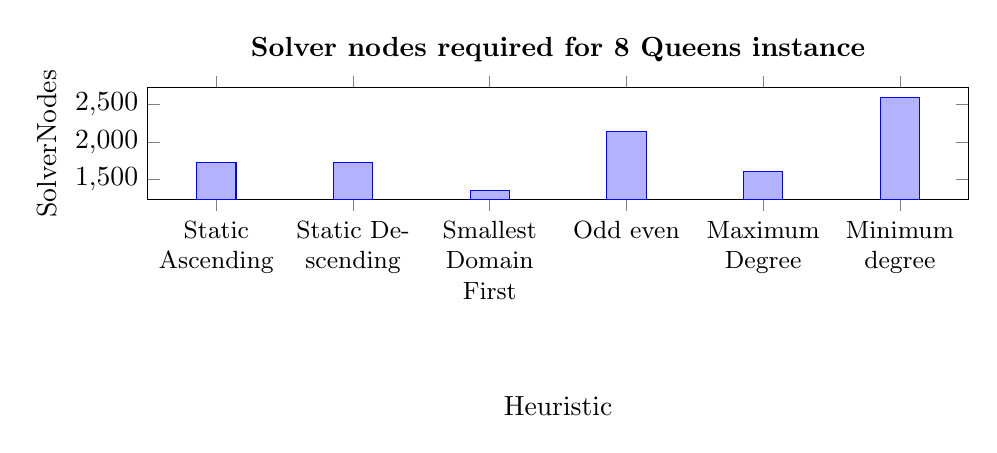
\begin{tikzpicture}
\begin{axis}[
	title = {\textbf{Solver nodes required for 8 Queens instance}},
	bar width=0.5cm,
	ybar,
	legend pos=south east,
	%enlarge x limits=0.4,
	height=3cm,
	width=12cm,
	xlabel={Heuristic},
	%xtick={23,24},
	%xticklabels={langfords2-3, langfords2-4},
	xtick=data,
	symbolic x coords = {Static Ascending,Static Descending,Smallest Domain First,Odd even,Maximum Degree,Minimum degree},
	x tick label style={font=\small,text width=1.5cm,align=center},
	legend pos=outer north east,
	ylabel={SolverNodes},
	xlabel style={yshift=-1cm}
]

\addplot coordinates {(Static Ascending, 1724) (Static Descending, 1724) (Smallest Domain First, 1360) (Odd even, 2132) (Maximum Degree, 1612) (Minimum degree, 2592)};

\end{axis}
\end{tikzpicture}
\\
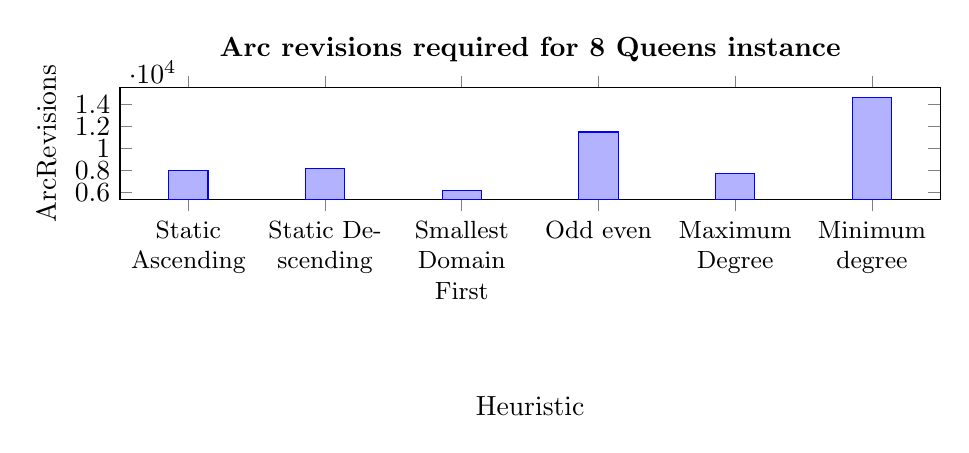
\begin{tikzpicture}
\begin{axis}[
	title = {\textbf{Arc revisions required for 8 Queens instance}},
	bar width=0.5cm,
	ybar,
	legend pos=south east,
	height=3cm,
	width=12cm,
	xlabel={Heuristic},
	xtick=data,
	symbolic x coords = {Static Ascending,Static Descending,Smallest Domain First,Odd even,Maximum Degree,Minimum degree},
	x tick label style={font=\small,text width=1.5cm,align=center},
	legend pos=outer north east,
	ylabel={ArcRevisions},
	xlabel style={yshift=-1cm}
]

\addplot coordinates {(Static Ascending, 7992) (Static Descending, 8162) (Smallest Domain First, 6168) (Odd even, 11472) (Maximum Degree, 7666) (Minimum degree, 14644)};
\end{axis}
\end{tikzpicture}
\\
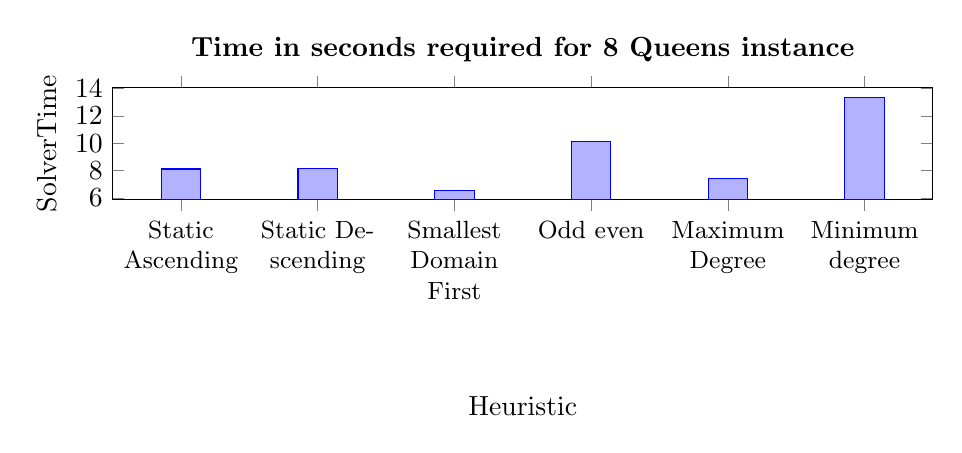
\begin{tikzpicture}
\begin{axis}[
	title = {\textbf{Time in seconds required for 8 Queens instance}},
	bar width=0.5cm,
	ybar,
	legend pos=south east,
	height=3cm,
	width=12cm,
	xlabel={Heuristic},
	xtick=data,
	symbolic x coords = {Static Ascending,Static Descending,Smallest Domain First,Odd even,Maximum Degree,Minimum degree},
	x tick label style={font=\small,text width=1.5cm,align=center},
	legend pos=outer north east,
	ylabel={SolverTime},
	xlabel style={yshift=-1cm}
]

\addplot coordinates {(Static Ascending, 8.12) (Static Descending, 8.18) (Smallest Domain First, 6.57) (Odd even, 10.1) (Maximum Degree, 7.46) (Minimum degree, 13.36)};
\end{axis}
\end{tikzpicture}
\caption{Performance of different heuristics on the 8-Queens problem. Heuristics that performance significantly worse such as largest domain first and random and excluded here.}
\end{figure}
\noindent
It was briefly touched on earlier than the random heuristic performed worse than all other heuristics, but not as badly as largest domain first. What is interesting to find out next is if there is a big difference between different random heuristics. This will further show which aspect of the heuristic is of more importance as different specific aspects are randomised. 

\begin{figure}[H]
\centering
\sixplot{N queens}{queens.csv}{\randomplot}
\caption{N queens problem performance of random heuristics}
\end{figure}
\noindent
From the four random heuristics tested, it can be seen clearly that the completely random heuristic and random variable heuristic perform worse. This shows two things:
\begin{enumerate}
\item Variable ordering is more important than value ordering in general - This is shown from the improved performance of random value ordering compared to the other three random heuristics, all of which included random variable ordering. The random value ordering was simply a static ascending order and its performance was not heavily impacted by the random value selection, as it took almost the same number of solver nodes and arc revisions as the completely static ascending heuristic. 
\item Having some form of order, even if a random order is better than always choosing randomly - By using a random static order, the same order is kept throughout solving the problem. The metrics measured for this approach is closely comparable to the odd even variable heuristic, showing how the two are almost equivalent, even from mixing up the order of the variables differently. Of course this may not apply to every problem, especially if a problem took advantage of an odd/even ordering, however, if it doesn't matter then a static random ordering is just as good. 
\end{enumerate}



\subsection{Langfords}
For langfords problem, multiple runs were not able to be completed easily due to the difficulty of the harder langfords (n = 3) problems taking too much time. As such, the time taken and random heuristics could not be measured for langfords problems where n \neq\ 2. Because the langfords problems for n = 3 are more difficult problems that take more search nodes and revisions, it is interesting to see how the heuristics are affected when the problems are more complex.  
\begin{figure}[H]
\centering
\begin{minipage}{0.45\textwidth}
\bargraph{Langfords}{Instance}{SolverNodes}{langfords.csv}{\legend{};}
\end{minipage}
%
\begin{minipage}{0.45\textwidth}
\bargraph{Langfords}{Instance}{ArcRevisions}{langfords.csv}{}
\end{minipage}
\caption{Langfords problem with different metrics and heuristics.}
\end{figure}
\noindent
For the smaller langfords problem, there is different pattern seen between the different heuristics. The best heuristic is a static descending order and the maximum degree ordering. This is different from the N-queens problem, where smallest domain first performed much better than all other heuristics. From this result, we can see that it is not always the case that dynamic heuristics like smallest domain first perform the best and static heuristics can be better depending on the problem and problem size. Here, the descending static order is able to perform well because the last variable is the hardest to search for. This is due to the properties of langford's problem, where the arrangement of the digits is important. Finding what the last digit is greatly helps reduce the domains needed to search which is why descending works well. Maximum degree is able to find the same performance because the last variable is the most constrained and so it also solves in descending order. Smallest domain first alone does not help as each variable has the same domain and the heuristic cannot infer any more information that can help it improve. 
\n
The graphs of the random heuristics show a similar pattern to the N-queens problem. The variable assignments can be seen to have a greater impact, as fully random and random variable ordering is much worse than a random static and random value ordering. 
\begin{figure}[H]
\centering
\begin{minipage}{0.45\textwidth}
\bargraphrandom{Langfords}{Instance}{SolverNodes}{langfords.csv}{\legend{};}
\end{minipage}
%
\begin{minipage}{0.45\textwidth}
\bargraphrandom{Langfords}{Instance}{ArcRevisions}{langfords.csv}{}
\end{minipage}
\caption{Langfords problem with random heuristics.}
\end{figure}
\noindent
The data for langfords of n = 3 further supports the fact that the descending static ordering performs better. However, running the maximum degree heuristic does not finish in time, which is strange. We can see the static descending order is significantly better than smallest domain first and ascending static order. The time taken is not very reliable as only one run was done, but the difference can clearly be seen. The strange issue is why the maximum degree heuristic was not able to finish in time. Perhaps this had to do with memory issues, or overhead before the solver started. However this does show that even if the heuristic should theoretically perform better, it is not always the case in practice due to other forms of overhead. 

\begin{figure}[H]
\centering
\begin{minipage}{0.45\textwidth}
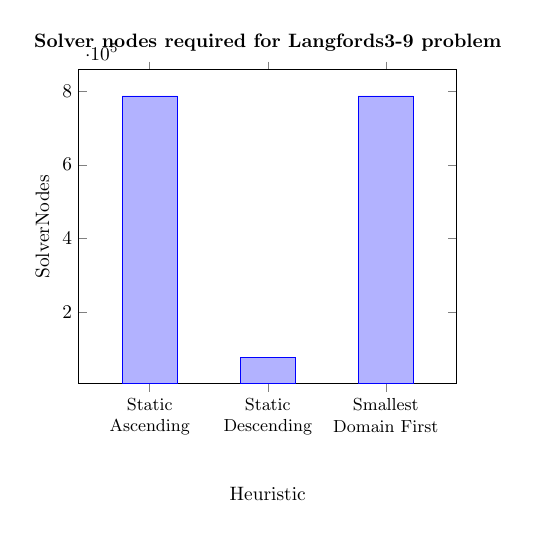
\begin{tikzpicture}[scale=0.7]
\begin{axis}[
	title = {\textbf{Solver nodes required for Langfords3-9 problem}},
	bar width=1cm,
	enlarge x limits=0.3,
	ybar,
	legend pos=south east,
	xlabel={Heuristic},
	xtick=data,
	symbolic x coords = {Static Ascending,Static Descending,Smallest Domain First},
	x tick label style={font=\small,text width=2cm,align=center},
	legend pos=outer north east,
	ylabel={SolverNodes},
	xlabel style={yshift=-0.7cm}
]

\addplot coordinates {(Static Ascending, 785991) (Static Descending, 78369) (Smallest Domain First, 785991)};
\end{axis}
\end{tikzpicture}
\end{minipage}
%
\begin{minipage}{0.45\textwidth}
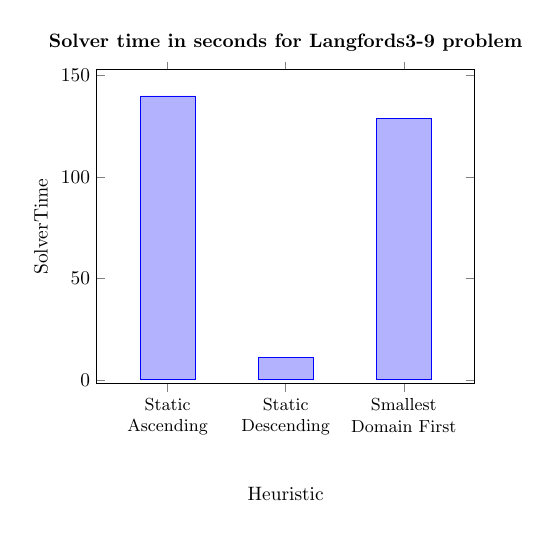
\begin{tikzpicture}[scale=0.7]
\begin{axis}[
	title = {\textbf{Solver time in seconds for Langfords3-9 problem}},
	bar width=1cm,
	ybar,
	enlarge x limits=0.3,
	legend pos=south east,
	xlabel={Heuristic},
	xtick=data,
	symbolic x coords = {Static Ascending,Static Descending,Smallest Domain First},
	x tick label style={font=\small,text width=2cm,align=center},
	legend pos=outer north east,
	ylabel={SolverTime},
	xlabel style={yshift=-0.7cm}
]

\addplot coordinates {(Static Ascending, 140) (Static Descending, 11) (Smallest Domain First, 129)};
\end{axis}
\end{tikzpicture}
\end{minipage}
\caption{Comparison of heuristics for Langfords3-9, showing the significant improvement of a static descending heuristic.}
\end{figure}

\subsection{Sudoku}
The two sudoku problems (SimonisSudoku and FinnishSudoku) are two of the harder problems to solve. In particular, many heuristics could not solve the FinnishSudoku problem in any reasonable amount of time, long enough that little comparison could have been made. Like the Langford's problem, because of the time needed to solve the sudoku problems, multiple runs for experimentation could not be done, and so the random heuristics and time taken are not analysed. For FinnishSudoku, no heuristic except for smallest domain first was able to finish in reasonable time which shows the strength in that particular heuristic.
\n
Furthermore, the following heuristics did not complete the SimonisSudoku in any reasonable time:
\begin{itemize}
\item Fully random and random variable heuristics
\item Maximum degree ordering
\item Largest domain first
\end{itemize}
Perhaps for the sudoku problem, the least constrained variables are better suited to being solved first, which would explain why the maximum degree could not finish when the minimum degree ordering finished quite quickly. 

\subsubsection*{Simonis Sudoku}
In the graphs for the SimonisSudoku problem instance, it can be seen that the odd/even static ordering took considerably more nodes and arc revisions than all other heuristics. This is due to the way the sudoku problem is modelled. Solving all odd then even variables makes it difficult to solve entire rows and columns. In fact no full row or column will be completed until all odd variables are assigned, as the odd even heuristic will go through the variables in a diagonal pattern, causing a lot of backtracking and wipeouts. Further, the random static heuristic also performed poorly, as its order was random, meaning some rows and columns may not be solved or finished until much later. In comparison, all the other methods which stuck to a ascending or descending order got much better results. 
\begin{figure}[H]
\centering
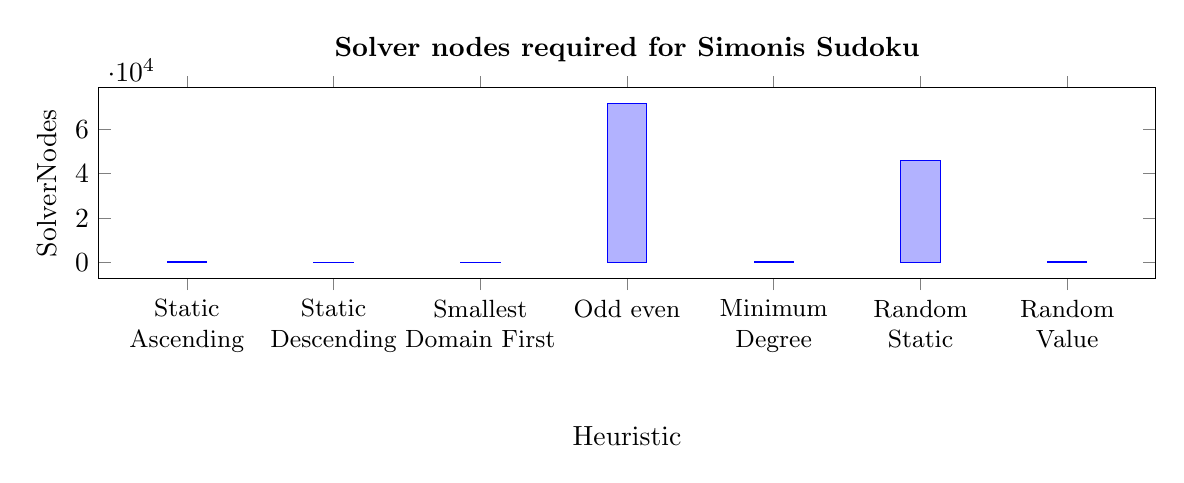
\begin{tikzpicture}
\begin{axis}[
	title = {\textbf{Solver nodes required for Simonis Sudoku}},
	bar width=0.5cm,
	width=15cm,
	height=4cm,
	ybar,
	enlarge x limits=0.1,
	legend pos=south east,
	xlabel={Heuristic},
	xtick=data,
	symbolic x coords = {Static Ascending,Static Descending,Smallest Domain First,Odd even,Minimum Degree,Random Static,Random Value},
	x tick label style={font=\small,text width=2cm,align=center},
	legend pos=outer north east,
	ylabel={SolverNodes},
	xlabel style={yshift=-0.7cm}
]

\addplot coordinates {(Static Ascending, 382) (Static Descending, 247) (Smallest Domain First, 81) (Odd even, 71477) (Minimum Degree, 398) (Random Static, 46142) (Random Value, 382)};
\end{axis}
\end{tikzpicture}
\\
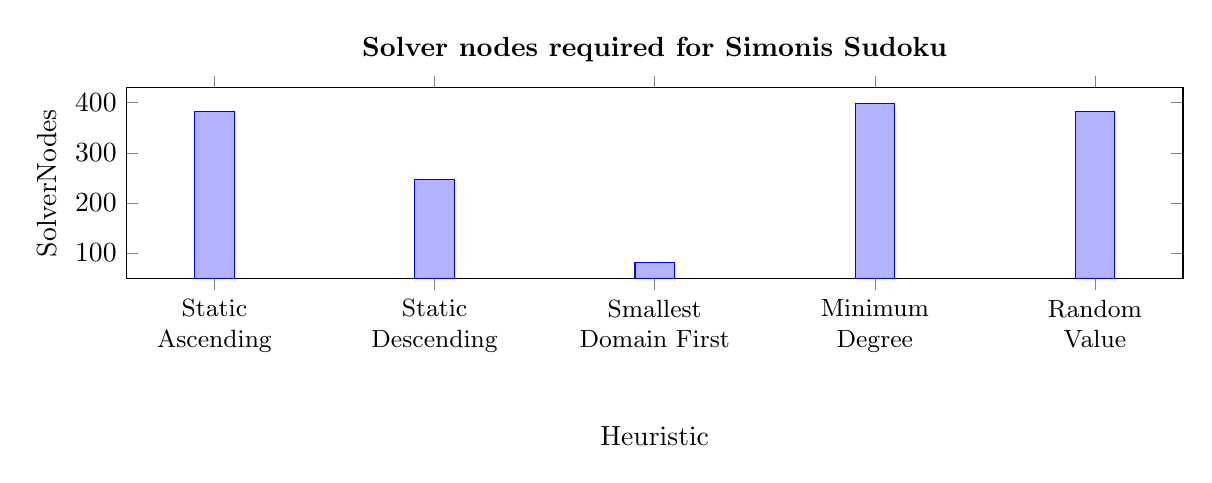
\begin{tikzpicture}
\begin{axis}[
	title = {\textbf{Solver nodes required for Simonis Sudoku}},
	bar width=0.5cm,
	width=15cm,
	height=4cm,
	ybar,
	enlarge x limits=0.1,
	legend pos=south east,
	xlabel={Heuristic},
	xtick=data,
	symbolic x coords = {Static Ascending,Static Descending,Smallest Domain First,Minimum Degree,Random Value},
	x tick label style={font=\small,text width=2cm,align=center},
	legend pos=outer north east,
	ylabel={SolverNodes},
	xlabel style={yshift=-0.7cm}
]

\addplot coordinates {(Static Ascending, 382) (Static Descending, 247) (Smallest Domain First, 81) (Minimum Degree, 398) (Random Value, 382)};
\end{axis}
\end{tikzpicture}
\caption{Solver nodes for Simonis Sudoku. The second graph does not show the odd even and random static heuristics for better comparison of the other five heuristics.}
\label{fig:simonis1}
\end{figure}


\begin{figure}[H]
\centering
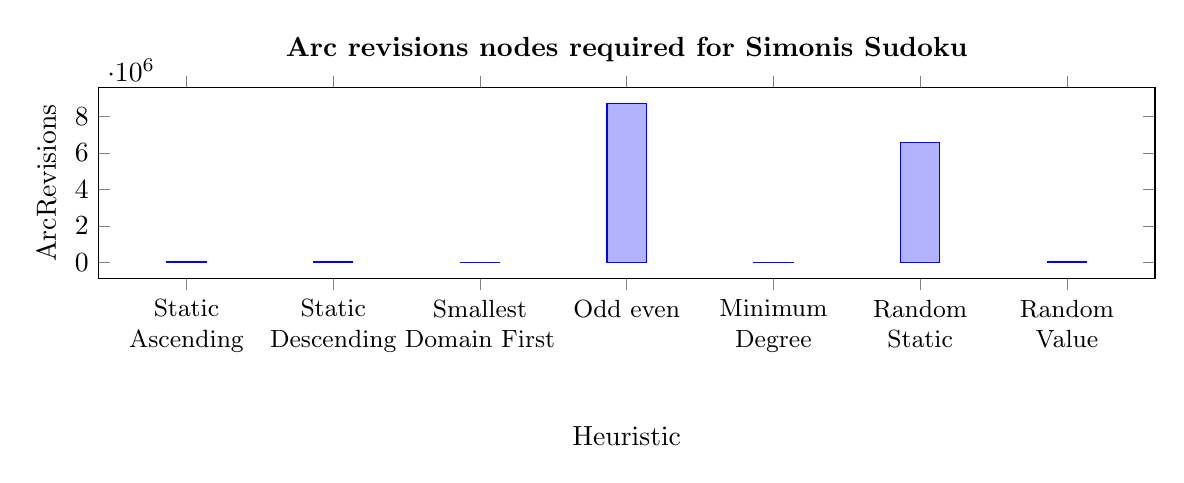
\begin{tikzpicture}
\begin{axis}[
	title = {\textbf{Arc revisions nodes required for Simonis Sudoku}},
	bar width=0.5cm,
	width=15cm,
	height=4cm,
	ybar,
	enlarge x limits=0.1,
	legend pos=south east,
	xlabel={Heuristic},
	xtick=data,
	symbolic x coords = {Static Ascending,Static Descending,Smallest Domain First,Odd even,Minimum Degree,Random Static,Random Value},
	x tick label style={font=\small,text width=2cm,align=center},
	legend pos=outer north east,
	ylabel={ArcRevisions},
	xlabel style={yshift=-0.7cm}
]

\addplot coordinates {(Static Ascending, 32142) (Static Descending, 28841) (Smallest Domain First, 3240) (Odd even, 8689977) (Minimum Degree, 17364) (Random Static, 6551838) (Random Value, 32142)};
\end{axis}
\end{tikzpicture}
\\
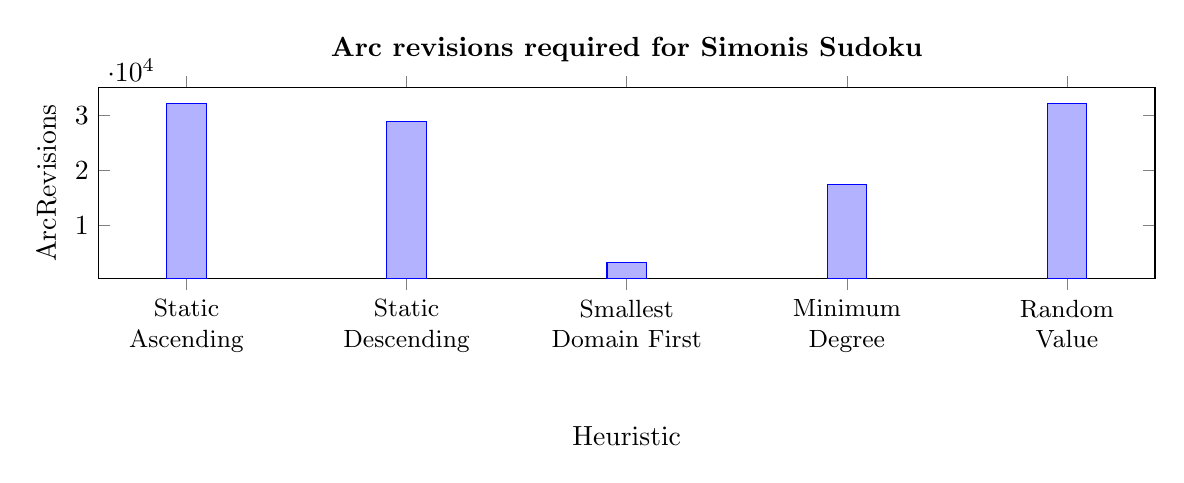
\begin{tikzpicture}
\begin{axis}[
	title = {\textbf{Arc revisions required for Simonis Sudoku}},
	bar width=0.5cm,
	width=15cm,
	height=4cm,
	ybar,
	enlarge x limits=0.1,
	legend pos=south east,
	xlabel={Heuristic},
	xtick=data,
	symbolic x coords = {Static Ascending,Static Descending,Smallest Domain First,Minimum Degree,Random Value},
	x tick label style={font=\small,text width=2cm,align=center},
	legend pos=outer north east,
	ylabel={ArcRevisions},
	xlabel style={yshift=-0.7cm}
]

\addplot coordinates {(Static Ascending, 32142) (Static Descending, 28841) (Smallest Domain First, 3240) (Minimum Degree, 17364) (Random Value, 32142)};
\end{axis}
\end{tikzpicture}
\caption{Arc revisions for Simonis Sudoku. The second graph does not show the odd even heuristic for better comparison of the other four heuristics.}
\end{figure}
\noindent
There are two more interesting points in the results for Simonis Sudoku. First, smallest domain first used the least number of revisions and solver nodes. This is similar to the N-queens problem, but contrasts with Langford's problem. This shows us that the performance of static heuristics can be very problem dependent, more so than dynamic heuristics. The is especially true the more specific a static heuristic is to a problem class, or even to a problem instance, as a static ordering can give the exact ordering of variables needed that gives the optimal search. Second, the minimum degree ordering gives more solver nodes relative to the other heuristics, but less arc revisions. This is the first case in our results where the number of nodes and revisions do not tell the exact same results. This is interesting as it means the minimum degree heuristic has a lower arc revision to search node ratio, so less revisions are done on average per branch, but more branching is done in general. This is good as it shows just looking at revisions or solver nodes it not necessarily a good enough indicator of performance. Moreover, the means the minimum degree heuristic has pruned less values, becomes more nodes had to be searched, but the additional search nodes did not require much revision.

\section{Conclusion}
In conclusion, a forward checking constraint solver was implemented. The solver was implemented to be able to take in any generic heuristic for variable and value section. Tests were written on the provided constraint satisfaction problem instances to ensure the correct number of all solutions could be found, verifying the correctness of the solver. 
\n
Next, different heuristics were implemented for the solver to use, which included a dynamic variable heuristic (smallest domain first) and static variable heuristics such as maximum degree. Further, random heuristics were tested to show the different affect of variable and value selection. 
\n
Finally, the heuristics were run on the various different problems where the time taken, number of solver nodes and number of arc revisions were measured to show the difference between the heuristics, especially the difference between a dynamic heuristic like smallest domain first, and a static heuristic like maximum degree. When looking at the N-queens problem, it appeared that static heuristics did not perform as well as dynamic heuristics. However, the Langfords' problems showed that this was not always the case, as a descending static order was able to perform significantly better than a smallest domain first heuristic. This demonstrated that a good static order built for specific problems could perform very well, but would be highly problem dependent while dynamic heuristics like smallest domain first could work well in most general cases. TODO sudoku


\printbibliography

\end{document}



